%!TEX root=../../../template.tex
\subsection{\acrlong{UAV}}%
\label{sub:methods_uav}

Although it was not possible to assemble the final physical system onto
an actual drone, I have managed to specify it completely in a custom
design for which Figure~\ref{fig:img/pdf/drone_schematic} is a basic
schematic~\footnote{To the reader: although this is still a fairly
advanced design, recent advances in drone technology might render it
a bit obsolete in some aspects. Please bear in mind that this design
was finished in March 2019}.

\begin{figure}[htpb]
    \centering
    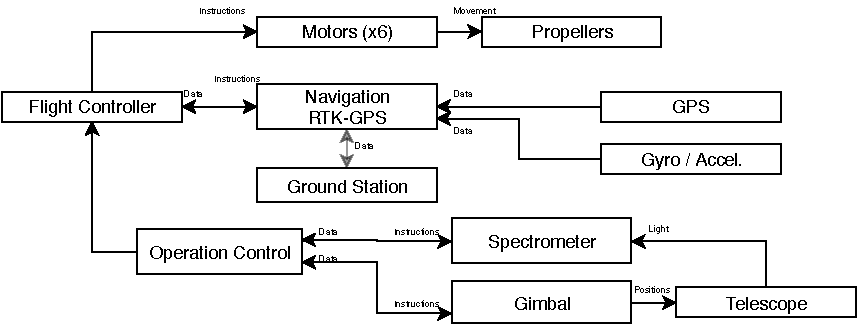
\includegraphics[width=0.8\linewidth]{img/pdf/drone.pdf}
    \caption{A schematic for the custom-designed drone system on which
    the pollution monitoring system would be mounted.}%
    \label{fig:img/pdf/drone_schematic}
\end{figure}

Our flight time requirements are between 30 to 40 minutes for each
measurement cycle. During this time, the drone would have to carry
itself and the collection equipment while still being able to land in a
safe position before recharging or replacing the batteries. Sufficiently
capable commercial systems were prohibitively expensive, thus I had to
design my own drone.

I began by selecting the type of drone I would use. Hexacopter models
are known around enthusiasts to be more efficient and stable, especially
if there is a high-payload requirement. They have several advantages
over the more "traditional" quadcopter designs. The most important is
certainly the fact that they can fly and land safely in case of one or
even two motors malfunctioning. Moreover, they are much stabler than
their 4 motor counterpart, and they are for the most part immune to (up
to) moderate winds. Finally, they are able to climb higher, since they
are less affected by thin air. They also have disadvantages, such as
their steeper cost, their size and their inherently higher complexity.
These drawbacks were easily manageable though, through the European
funds of project \gls{ATMOS} and the technical abilities of the team in
which the project was being developed.

I have therefore settled on a DJI S900 frame. This was, at the time of
selection, being discontinued by the Chinese brand. However, this model
remained popular among custom builders because of the familiarity people
already had with it and the fact that is was still commonly available in
specialised retailers. I was advised by two specialists to increase the
device's breadth through the addition of custom made 368mm arms. This
inclusion served two purposes: on the one hand, it reduced weight, since
the original arms were made of aluminium and the new ones were carbon
fibre; on the other hand, they granted the room needed for wider
propellers, with 17" blades. To accommodate the change in propeller
size, it was also advisable to replace the original motors by more
powerful units. In this case, I chose the DJI E1200. Larger propellers,
lighter body and more powerful motors led to significant improvements in
both flight time and carrying capacity. According to the manufacturer,
this configuration is able to handle a maximum weight per rotor of
3900g, or almost 24 kg in total. Assuming our drone to weight 6 kg, this
gives us a very comfortable weight margin for our payload, which in any
case should be slightly below 2 kg~\cite{DJI2015}.

A Pixhawk flight controller takes care of the aerial dynamics, movement
and positioning. This flight controller comes with all the needed
sensors (gyroscopes, barometers, magnetometers, accelerometers, etc.),
requiring only an external navigation unit. The unit natively supports
\gls{RTK-GPS}, a combination of inertial sensors and traditional
satellite navigation data that achieves positioning precisions of a few
tens of centimetres~\cite{Zimmermann2017, Triantafyllou2011}.

